\documentclass[draft=false
              ,paper=a4
              ,twoside=false
              ,fontsize=11pt
              ,headsepline
              ,BCOR10mm
              ,DIV11
              ]{scrbook}
\usepackage[ngerman,english]{babel}
%% see http://www.tex.ac.uk/cgi-bin/texfaq2html?label=uselmfonts
\usepackage[T1]{fontenc}
\usepackage[utf8]{inputenc}
%\usepackage[latin1]{inputenc}
\usepackage{libertine}
\usepackage{pifont}
\usepackage{microtype}
\usepackage{textcomp}
\usepackage[german,refpage]{nomencl}
\usepackage{setspace}
\usepackage[xindy]{imakeidx}
\usepackage{listings}
%%\usepackage{natbib}
\usepackage[ngerman,hidelinks]{hyperref}
\usepackage{soul}
\usepackage{hawstyle}
\usepackage{lipsum} %% for sample text
\usepackage{etoolbox}
%% All my packages
\definecolor{grey}{HTML}{E6E6E6}
\usepackage{realboxes}
\usepackage{amsmath}
\usepackage{framed}
\usepackage[amsmath,standard,hyperref,framed]{ntheorem}
\usepackage{tabu}
\usepackage{multirow}
\usepackage{pgf-umlsd}
\usepackage{bytefield}
\usepackage{float}
\usepackage{csquotes}
\usepackage[sorting=none,backend=biber,citestyle=numeric,doi=true,url=true]{biblatex}
\addbibresource{sample.bib}
%%\usepackage{amsthm}
\usepackage{parskip}

\usepackage{siunitx}
\sisetup{detect-all = true, free-standing-units = true}
%%\usepackage{xindy}
\usepackage[toc,acronym,xindy]{glossaries}

%%\usepackage{tocloft}
\usepackage{tocbibind}
\graphicspath{{./res/}{./logo/}}

\newacronym{tap}{TAP}{Test access port}
\newacronym{dap}{DAP}{Debug access port}
\newacronym{ide}{IDE}{Integrated Development Environment}
\newacronym{gdb}{GDB}{GNU Debugger}
\newacronym{swd}{SWD}{Serial Wire Debug}
\newacronym{jtag}{JTAG}{Joint Test Action Group}
\newacronym{isp}{ISP}{In-System Programmer}
\newacronym{cpu}{CPU}{Central Processing Unit}
\newacronym{uml}{UML}{Unified Modeling Language}
\newacronym{uart}{UART}{Universal Asynchronous Receiver Transmitter}
\newacronym{ntp}{NTP}{Network Time Protocol}
\newacronym{rom}{ROM}{Read-Only Memory}
\newacronym{ic}{IC}{Integrated Circuit}
\newacronym{gpio}{GPIO}{General purpose input/output}
\newacronym{uci}{UCI}{Unified Configuration Interface}
\newcommand{\listinlsh}[1]{\Colorbox{grey}{\lstinline[language=sh]{#1}}}
\newcommand{\listinlcpp}[1]{\Colorbox{grey}{\lstinline[language=C++]{#1}}}
\newcommand{\listinljava}[1]{\Colorbox{grey}{\lstinline[language=Java]{#1}}}
%%\theoremstyle{definition}
%%\newtheorem{defi}{Definition}
%%\theoremindent9pt
\theoremprework{\par\begin{minipage}{\textwidth}\hrule\medskip}
\theorempostwork{\hrule\medskip\end{minipage}}
%%\renewtheoremstyle{definition}
\renewtheorem{definition}{Definition}[chapter]
%%\newacronym{dap}{DAP}{Debug access port}
%%\newacronym{tap}{TAP}{test access port}
\makeglossaries
%%\renewcommand{\cftdot}{.}
%%\renewcommand*{\familydefault}{\sfdefault}
\makeatletter
%%\patchcmd{\chapter}{\if@openright\cleardoublepage\else\clearpage\fi}{\par}{}{}
\renewcommand\fs@ruled{\def\@fs@cfont{\bfseries}\let\@fs@capt\floatc@ruled
%%\def\@fs@post{\hrule height.8pt depth0pt \kern2pt}%
\def\@fs@post{\relax}
\def\@fs@pre{\kern2pt\hrule\kern8pt}%
\def\@fs@mid{\kern8pt\hrule\kern2pt}%
\let\@fs@iftopcapt\iffalse}
\makeatother
\usepackage{minitoc}
%% define some colors
\colorlet{BackgroundColor}{gray!20}
\colorlet{KeywordColor}{blue}
\colorlet{CommentColor}{black!60}
%% for tables
\colorlet{HeadColor}{gray!60}
\colorlet{Color1}{blue!10}
\colorlet{Color2}{white}

%% configure colors
\HAWifprinter{
  \colorlet{BackgroundColor}{gray!20}
  \colorlet{KeywordColor}{black}
  \colorlet{CommentColor}{gray}
  % for tables
  \colorlet{HeadColor}{gray!60}
  \colorlet{Color1}{gray!40}
  \colorlet{Color2}{white}
}{}
\lstset{%
  numbers=left,
  numberstyle=\tiny,
  stepnumber=1,
  numbersep=5pt,
  basicstyle=\ttfamily\small,
  keywordstyle=\color{KeywordColor}\bfseries,
  identifierstyle=\color{black},
  commentstyle=\color{CommentColor},
  backgroundcolor=\color{BackgroundColor},
  captionpos=b,
  fontadjust=true
}
\lstset{escapeinside={(*@}{@*)}, % used to enter latex code inside listings
        morekeywords={uint32_t, int32_t}
}
\ifpdfoutput{
  \hypersetup{bookmarksopen=false,bookmarksnumbered,linktocpage}
}{}

%% more fancy C++
\DeclareRobustCommand{\cxx}{C\raisebox{0.25ex}{{\scriptsize +\kern-0.25ex +}}}

\clubpenalty=10000
\widowpenalty=10000
\displaywidowpenalty=10000

% unknown hyphenations
\hyphenation{
}

%% recalculate text area
\typearea[current]{last}

\makeindex
\makenomenclature

\begin{document}
\selectlanguage{ngerman}
\floatstyle{ruled}
\restylefloat{figure}
%%%%%
%% customize (see readme.pdf for supported values)
\HAWThesisProperties{Author={Arne Wischer	}
                    ,Title={Design und Implementierung eines verteilten
                    linuxbasierten Entwicklungssystems für
                    Nahbereichsfunkanwendungen mit ARM-Architektur }
                    ,EnglishTitle={Developing software in Germany}
                    ,ThesisType={Bachelorarbeit}
                    ,ExaminationType={Bachelorprüfung}
                    ,DegreeProgramme={Bachelor of Science Technische Informatik} ,ThesisExperts={Prof. Dr. rer. nat. Hans Heinrich Heitmann \and Prof.
                    Dr.
                    Zweitprüfer} ,ReleaseDate={18. April 2013}
                  }

%% title
\frontmatter
%%Grobstruktur der Arbeit
\begin{itemize}
  \item Einführung
  \begin{itemize}
    \item Motivation - Eingebettete Systeme behrrschen unseren Alltag. Funk ist
    allgegenwärtig in Heim und Industrie
    \item Ziele - Eine Möglichkeit ein System zu planen, entwerfen und
    umzusetzen.
    \item Gliederung - Wie diese Arbeit aufgebaut ist
  \end{itemize}
  \item Analyse
  \begin{itemize}
    \item Grundidee - wie das System aufgebaut werden soll. (Bild)
    \item Bestandteile einer (allgemeinen) Entwicklungsplattform analysieren
    (Vorgehensmodell, Software, Hardware)
    \item Vorgaben - Funk, ARM, linuxbasiert
    \item Vorentscheidungen - Olimex ARM, Olimex-Funk, Carambola
    \item Anforderungen - Welche Punkte erfüllt werden müssen: Debugging,
    Analyse von zentral gesammelten (Funk-)Daten, Deployment einer Anwendung
  \end{itemize}
  \item Konzeption
  \begin{itemize}
    \item Debugging
    \begin{itemize}
      \item Was Debugging bedeutet, welche Bestandteile benötigt werden
      \item Was existiert - OpenOCD, ZY1000, sonstige
      Debugger? => Anpassung von OpenOCD an OpenWRT
      \item Cross-Compilierung
      \item OpenWRT Paketverwaltung - 
      \item Wahl eines JTAG Adapters
      \item Zielsetzung für das Debugging
  	\end{itemize}
  	\item Datenanalyse
  	\begin{itemize}
  	  \item Anforderungen - Zusammenführung von Daten, Zeitlicher Ablauf
  	  erkennbar
  	  \item Bestandteile - Client, Server, Protokoll um beides zu verbinden
  	  \item Zeitsynchronisation - NTP, Ablaufdiagramm
      \item Protokoll - Tabelle, Erläuterung
    \end{itemize}
    \item Deployment
    \begin{itemize}
      \item Flashen einer Firmware
      \item Nutzung von JTAG
    \end{itemize}
  \end{itemize}
  \item Realisierung
  \begin{itemize}
    \item OpenOCD
    \item Server(C++-Programm)
    \item Client(Java-Programm)
    \item Deployment(Skript)
  \end{itemize}
  \item Ausblick/Erweiterungsmöglichkeiten
\end{itemize}
\setcounter{page}{0}
%% output title page
\maketitle

\onehalfspacing

%% add abstract pages
%% note: this is one command on multiple lines
\HAWAbstractPage
%% German abstract
{Schlüsselwort 1, Schlüsselwort 2}%
{Dieses Dokument \ldots}
%% English abstract
{keyword 1, keyword 2}%
{This document \ldots}

\newpage
\singlespacing
\mtcselectlanguage{german}
\dominitoc
\tableofcontents

\newpage
%% enable if these lists should be shown on their own page
%%\listoftables
%%\listoffigures
%\lstlistoflistings
\printglossary[type=acronym,title=Abkürzungsverzeichnis,toctitle=Abkürzungsverzeichnis]
%%\printglossaries
\adjustmtc
%% main
\mainmatter
\onehalfspacing
%% write to the log/stdout

\typeout{===== File: chapter 1}
%% include chapter file (chapter1.tex)o
\chapter{Einführung}
\adjustmtc
\minitoc
\section{Motivation}
Eingebettete Systeme sind aus unseren heutigen Welt nicht mehr wegzudenken. Sie
dienen zur Heimautomatisierung, Prozesssteuerung und vielem
Anderen. Diese Systeme kommunizieren häufig über Funkprotokolle, die auf eine
hohe Energieeffizienz ausgelegt sind und sich in ihrem Netzwerkaufbau oftmals
dynamisch organisieren können. Als Beispiel für derartige Funksysteme lassen
sich \emph{ZigBee}, \emph{ANT}, \emph{Z-Wave}, \emph{Bluetooth low energy} oder
\emph{MiWi} nennen.

Gleichzeitig sind diese Systeme stark in bestehende Umgebungen wie Anlagen oder
Bausubstanz integriert beziehungsweise müssen in eine solche Umgebung
integriert werden.

Die Problematik liegt hierbei in der Entwicklung dieser vernetzten Systeme. Wird
ein einzelnes System entwickelt, sind die Randbedingungen meist recht klar
definiert, Anwendungen zur Softwareentwicklung sind weit verbreitet und gängige
Testverfahren können die Einhaltung der Vorgaben überprüfen.

Soll jedoch ein Funknetzwerk, bestehend aus mehreren einzelnen Systemen,
entwickelt werden, offenbaren sich manche Schwierigkeiten erst im
Zusammenspiel der einzelnen Komponenten. Auch können störende
Umwelteinflüsse in der Konzeption nicht unbedingt immer vollständig erfasst und
bedacht werden.

Dazu kommt, dass meist eine Vielzahl identischer Systeme miteinander
kommuniziert und so auch oft die gleiche Software auf diesen Systemen zum
Einsatz kommt.

Und auch eine fortlaufende Wartung dieser Systeme ist, aufgrund der teilweise
hohen räumlichen Abstände, nicht immer sehr einfach zu handhaben. 

\section{Existierende Lösungen}\label{sec:exist}
Für stark in ihren Ressourcen eingeschränkte, verteilte Funksysteme existieren
eine Anzahl hierfür optimierter Betriebssysteme. Das TinyOS-Projekt\cite{TINY}
zum Beispiel ist ein an der Universität Berkeley entstandenes und spezifisch für
den Betrieb drahtloser Sensornetzwerke entwickeltes Betriebssystem. Weitere
Beispiele wären Contiki\cite{CONT} oder FreeRTOS\cite{FREE}.

Die meisten dieser Betriebssysteme benötigen zum Ändern oder
Aktualisieren der Firmware eine direkte Verbindung zu dem Rechner des
Entwicklers. Dies kann, insbesondere mit einer Hohen Anzahl Sensorknoten,
durchaus zu einer logistischen Herausforderung werden.

\begin{definition}[Zielsystem]
Das \emph{Zielsystem} ist das System, welches mit Hilfe des
\emph{Entwicklungssystems} realisiert werden soll.
\end{definition}

Um dieses Problem zu umgehen, verfolgt TinyOS einen anderen Ansatz. Will man auf
mehrere TinyOS-basierte Zielsysteme beziehungsweise Sensorknoten eine neue
Softwareversion aufspielen, kann man sich die in das System integrierte Software
"`Deluge 2"'\cite{DELUG} zunutze machen. Diese Software ermöglicht es, eine neue
Softwareversion mittels eines Bootloaders und über das bereits bestehende
Funknetzwerk zu verteilen. Hierbei funktioniert die Verteilung "`epidemisch"'
und wird damit größtenteils durch die Sensorknoten selbst verwaltet.

Dieses Vorgehen hat jedoch wiederum den Nachteil, dass für eine Verteilung der
Software überhaupt erst einmal ein Netzwerk unter den Sensorknoten existieren
muss. So wird dieses Verfahren unmöglich, sobald ein komplett neues
Funkprotokoll entwickelt werden soll.

Wünschenswert wäre es also, die Verteilung neuer Softwareversionen möglichst
kabellos und gkeichzeitig ohne starke Abhängigkeit vom Zielsystem oder dem
verwendeten Funksystem durchführen zu können.

Während der Entwicklung eines solchen Funksystems spielen auch andere
Aspekte eine Rolle. So ist es ab einem gewissen Punkt in der Entwicklung sicher
wichtig, diese Systeme und die Abläufe im Funknetz im laufenden Betrieb
analysieren zu können.

\section{Ziele}
Ziel dieser Bachelorarbeit ist es, ein Entwicklungssystem zu schaffen,
mit dessen Hilfe sich integrierte und mit einem Funkmodul ausgestattete
Zielsysteme entwickeln und in ihrem Betrieb untersuchen lassen.

Hierzu werden verschiedene Hilfsmittel benötigt, deren einzelne Bestandteile
herausgearbeitet, entworfen und implementiert werden sollen.
\section{Gliederung}
Im ersten Teil werden bestehende Systeme analysiert, um <\ldots>

\chapter{Analyse eines Entwicklungssystems}\label{chap:analyse}
\minitoc
In diesem Kapitel soll aufgezeigt werden, woraus ein Entwicklungssystem
im Allgemeinen besteht und welche Anforderungen sich also für ein zu
entwerfendes Entwicklungssystem ergeben.
\section{Begriffsdefinitionen}
\subsection*{Zielsystem}
Das \emph{Zielsystem} ist das zu entwerfende Entwicklungsziel.
\subsection*{Entwicklungsplattform}
Zu einer \emph{Entwicklungsplattform} gehören alle Hardware- und
Softwareelemente, die nötig sind, um die Umsetzung eines bestimmten
Softwareprojektes zu erreichen. Die einzelnen Bestandteile einer solchen
\emph{Entwicklungsplattform} sollen im Verlauf dieses Kapitels identifiziert
werden.
\section{Elemente einer Entwicklungsplattform}
Die Elemente einer Entwicklungsplattform lassen sich grob drei Kategorien
zuordnen. 
\subsection{Vorgehensmodell}
Zu jedem Entwicklungsprozesses gehört auch immer die Entscheidung über eine
Vorgehensweise. Viele Vorgehensweisen basieren dabei auf Vorgehensmodellen,
die in Industrie und Wirtschaft weit verbreitet sind. Als Beispiele lassen sich
hier das Wasserfallmodell, das V-Modell, Scrum oder auch Extreme Programming
nennen.

All diesen Modellen ist gemein, dass einige ihrer Schritte
unbedingt Unterstützung durch Soft- und Hardwareware bedürfen oder
diese die Entwicklung unter Umständen beschleunigen kann.
Einige Vorgehensmodelle sollen hier exemplarisch aufgeführt werden.
\subsubsection*{Wasserfallmodell}
Das Wasserfallmodell ist ein klassisches, nicht-iteratives Vorgehensmodell,
dessen Ablauf man sich anhand eines Wasserfalls gut visualisieren kann. 

\begin{figure}[!h]
\centering
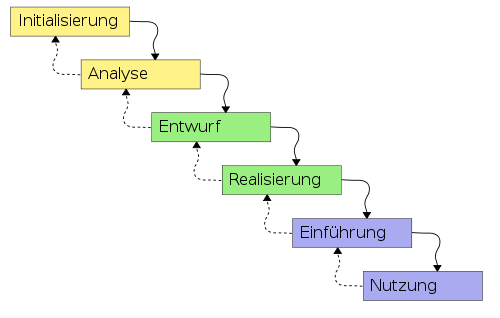
\includegraphics[width=350pt]{wasserfallmodell.png}
\caption{Ablauf eines Softwareprojektes nach dem Wasserfallmodell Aufgenommen:
12.03.2013}
\end{figure}

Jeder einzelne Schritt in der Entwicklung stellt hierbei eine abgeschlossene
Phase mit vorher festgelegten Anfangs- und Endpunkten dar.

In den Initialisierungs- und Analysephasen wird oft der Kunde in die
Entwicklung eingebunden. Typischerweise werden hier deshalb keine oder nur
wenige spezialisierte Tools verwendet.

Die Entwurfs- und Realisierungsphasen jedoch benötigen oft eine hohe
Softwareunterstützung. Während in der Entwurfsphase meist Tools zur
Visualisierung und Strukturierung von Softwarearchtiektur eingesetzt wird
(UML, Struktogramme, etc.) kann man Werkzeuge zur Planung und
Visualisierung von Soft

 \subsubsection*{Scrum} Scrum ist ein iteratives und agiles Modell zur
 Entwicklung von Software.
 
  \subsubsection*{Extreme Programming}
Hier Extreme Programming beschreiben

\subsection{Software}
Software unterstützt Softwareprojekte in allen Phasen der Durchführung.
\begin{itemize}
  \item \subsection*{IDEs} IDEs\footnote{Integrated Development Environment}
  sind zentrale Entwicklungsoberflächen der Softwareentwickler. In dieser
  Umgebung werden oftmals viele Tools zusammengefasst, die für den
  Entwicklungszyklus notwendig sind. Sie dienen dazu Quelltext zu verwalten,
  Versionsverwaltung zu betreiben, Code zu kompilieren, die entwickelte Software
  zu testen, zu deployen und zu debuggen.
  
  Oft werden die in den folgenden Punkten aufgeführten Tools in eine IDE
  integriert, um Entwicklungsabläufe zu vereinfachen und zu beschleunigen.
  
  \emph{Beispiele:} Eclipse, NetBeans, CodeWarrior, Microsoft Visual Studio, Qt
  Creator
  \item \subsubsection*{Compiler} Compiler sind für viele Softwareprojekte von
  essentieller Bedeutung. Speziell im eingebetteten Bereich werden überwiegend
  kompilierte Programmiersprachen wie C oder C++ eingesetzt, da sie nach dem
  Kompiliervorgang in nativem Maschinencode vorliegen und so oft eine höhere
  Ausführungsgeschwinidgkeit gewährleisten können. Außerdem können sie meist
  besser an das Zielsystem angepasst werden, da sie keiner weiteren Frameworks
  oder Interpreter mit "`überflüssigen"' Funktionen bedürfen.
  
  Soll eine kompilierte Software auf einem anderen als dem Entwicklungssystem
  eingesetzt werden, so wird ein sogenannter \textbf{Cross-Compiler} benötigt.
  Diese speziellen Compiler sind in der Lage, Software zu kompilieren, die
  später auf einer andere Rechnerarchitektur (z.B. ARM statt Intel) und/oder auf
  einem anderen Betriebssystem (z.B. Linux statt Windows) betrieben werden soll.
  
  \emph{Beispiele:} GCC, IAR C/C++ Compiler, ARM RVCT Compiler, Intel C++
  Compiler, CodeWarrior Compiler
  \item \subsubsection*{Debugger}
   Tool, um Software während seiner Laufzeit untersuchen zu können.
   
  \emph{Beispiele:} GDB
  \item \subsubsection*{Testtools}
  Tool, um Software auf Einhatung geforderter Parameter zu prüfen.
  
  \emph{Beispiele:} Unittests, , JTAG, SWD, 
  \item \subsubsection*{Deploymenttools}
  

  \emph{Beispiele:} Installer
\end{itemize}

\subsection{Hardware}
\begin{itemize}
  \item Hardware-Testtools
  \item Flasher
  \item ns
\end{itemize}
\subsection{Vorgehensmodell}
Zu jedem Entwicklungsprozesses gehört auch immer die Entscheidung über eine
Vorgehensweise. Viele Vorgehensweisen basieren dabei auf Vorgehensmodellen,
die in Industrie und Wirtschaft weit verbreitet sind. Als Beispiele lassen sich
hier das Wasserfallmodell, das V-Modell, Scrum oder auch Extreme Programming
nennen.

All diesen Modellen ist gemein, dass einige ihrer Schritte unbedingt
Softwareunterstützung bedürfen oder diese die Entwicklung unter
Umständen beschleunigen kann.
Einige Vorgehensmodelle und deren nötige Softwareunterstützung sollen hier
exemplarisch aufgeführt werden.
\subsubsection*{Wasserfallmodell}
Das Wasserfallmodell ist ein klassisches, nicht-iteratives Vorgehensmodell,
dessen Ablauf man sich anhand eines Wasserfalls gut visualisieren kann. 


\begin{figure}[h!]
\centering

\includegraphics[width=350pt]{HAW_logo}
\caption{Ablauf eines Softwareprojektes nach dem Wasserfallmodell}
\end{figure}

Jeder einzelne Schritt in der Entwicklung stellt hierbei eine abgeschlossene
Phase mit vorher festgelegten Anfangs- und Endpunkten dar.

 \subsubsection*{Scrum} Hier Scrum beschreiben
\subsubsection*{Extreme Programming}
Hier Extreme Programming beschreiben
\section{Softwareunterstützung}
Für eine neue Entwicklungsplattform ist es wünschenswert, sich nicht von einem
speziellen Vorgehensmodell abhängig zu machen. Es sollte also eine Schnittmenge
gefunden werden, um die Minimalanforderungen möglichst vieler Modelle abdecken
zu können.

Als Schnittmenge kristallisieren sich dabei folgende Aspekte heraus:
\begin{itemize}
  \item \subsection*{Programmieren} Eine Softwareunterstützung erfolgt in diesem
  Schritt meist durch eine IDE und/oder einen Compiler.
  \item \subsection*{Testen} Je nach Art der Tests wird auch in diesem Schritt
  Softwareunterstützung benötigt. 
  \item \subsection*{Verteilen} Soll eine Software auf mehrere
  Systeme verteilt werden, passiert dies fast immer softwaregestützt.
  \item \subsection*{Warten} Die Wartung einer Software ist ein weiterer
  wichtiger Bestandteil des Softwarelebenszyklus'.
\end{itemize}
\section{Vorbedingungen durch das zu entwickelnde System}\label{sec:vorb}
Entwicklung von Software für funkende Mikrocontroller. Dies Mikrocontroller sind
teilweise hochgradig in ihre Umgebung integriert. So können diese z.B.
nicht für die Entwicklung kurzfristig ausgebaut werden. Aufgrund ihrer extrem
hohen Verbreitung\footnote{Referenz} bezieht sich diese Arbeit ausschließlich
auf Systeme mit ARM-Architektur.
\section{Weitere Gegebenheiten}\label{sec:gegeb}
Es existiert Infrastruktur, die man sich für die Entwicklung zu Nutze machen
kann. Hierzu zählen zum Beispiel WLAN, Stromversorgung, Ethernet.

\section{Randbedingungen des Entwicklungsprozesses}
Die gegebenen Umständen aus \autoref{sec:gegeb} und \autoref{sec:vorb} ergeben
folgende Randbedingungen:
\begin{itemize}
  \item Das Zielsystem ist nie auch gleichzeitig das Entwicklungssystem.
  Zusätzlich zu der Tatsache, dass die Zielsysteme eine andere
  \item Das Zielsystem interagiert mit Umgebung. Deshalb sind zum Beispiel
  Funkstörungen o.Ä. zu beachten
  \item Der Zielsystemort ist selten auch der Entwicklungsort
  \item Es existieren viele Zielsysteme mit gleicher oder ähnlicher
  Konfiguration
\end{itemize}

\section{Anforderungen an das Entwicklungssystem}
Aus den Randbedingungen ergeben sich harte und weiche Anforderungen an ein
potentielles Entwicklungssystem. Die harten Anforderungen müssen von einem
Entwicklungssytem zwangsweise erfüllt werden um als geeignetes System dienen zu
können. Die Erfüllung weicher Anforderungen kann den den
Entwicklungsprozess vereinfachen und dem Entwickler die Arbeit erleichtern.
\subsection{Harte Anforderungen}
\begin{itemize}
  \item Schon während der Entwicklung muss ein Zugriff auf das Zielsystem zum
  Debuggen möglich sein
  \item Software muss "`remote"' deployt werden können
  \item Tests sollten aus Simulationsgründen vor Ort erfolgen
  \item Wartungszyklen und Wartungsupdates müssen meist für viele Systeme
  parallel duchgeführt werden
\end{itemize}
\subsection{Weiche Anforderungen}
\begin{itemize}
  \item 
\end{itemize}


\section{Entwicklungsmodelle}
Unterschiedliche Anforderungen je nach Entwicklungsziel
Manche stimmen jedoch überein, so z.B.
  



Abhängig von den Vorfaben und den eingesetzten Entwicklungsmodellen werden
für jedes Softwareprojekt unterschiedliche Anforderungen an die verwendete Hard-
und Software gestellt.

Diese Anforderungen 

 Je nach Art der Software, Anforderungen und

Unabhängig von der Wahl des Entwicklungsmodells können und
müssen viele dieser Schritte teilweise auch softwaregestützt ablaufen. Es ist
daher für ein Entwicklungssystem zwingend notwendig, diese Schritte zu
unterstützten.

Zu den softwaregestützten Schritten zählen hierbei:
\begin{itemize}
  \item \subsection*{Modultest} Modultest
  \item \subsection*{Integrationstest} Integrationstest eingebetteter Systeme
  erfolgen meist mit Hilfe standardisierter Verfahren. Diese verfahren lassen
  sich oft auch zum Beispiel in die Endkontrolle von herstellungsprozessen
  integrieren. So sind in der Industrie verfahren wie JTAG oder Pintests weit
  verbreitet.
  \item \subsection*{Deployment} Im Bereich der 
  \item \subsection*{Wartung}
\end{itemize}

\ldots
\section{JTAG}
JTAG statt SWD
\begin{itemize}
  \item Wird von viele Prozessoren unterstützt.
  \item Ermöglicht ein umfangreiches Debuggen des Prozessors bis auf
		Registerebene.
  \item OpenOCD hat bereits viele Funktionen.
\end{itemize}
\section{Netzwerkprotokoll}
\subsection{Zeitsynchronisation}
\section{Serversoftware}

\section{Clientsoftware}

\lipsum
\chapter{Konzeption}
\minitoc
In diesem Kapitel soll das Entwicklungssystem konzipiert werden.
Dazu muss jedes Element auf seine zu erfüllende Funktion untersucht werden.

Hieraus ergibt sich im Anschluss der anzufordernde Funktionsumfang, den der
jeweilige Bestandteil zu erfüllen hat.

Nach einer Analyse bereits existierender Systeme folgt schließlich die
Festlegung auf ein Entwicklungsziel.

Letztendlich muss sichergestellt werden, dass alle einzelnen Komponenten in dem
zu planenden System miteinander interagieren. Es müssen
Schnittstellenspezifikationen festgelegt werden.
\section{Debugging}
\subsection{Definition}
Das Debugging eines eingebetteten Systems erfordert meist eine kombinierte Hard-
und Softwarelösung.

Der Softwareteil ist oft in die \gls{ide} des Entwicklers eingebunden oder lässt
sich zumindest vom Arbeitsplatz des Entwicklers aus steuern. Die Befehle des
Entwicklers (Setzen eines Breakpoints, Abfrage von Registerwerten, etc.) werden
vom Softwaretreiber anschließend in Steuerbefehle des Hardwarebauteils
umgesetzt. Das Hardwaremodul übernimmt hierauf, unter Nutzung eine
standardisierten Schnittstelle, die Kommunikation mit dem Zielsystem.

Als Schnittstellen sind für diese Zwecke vor allem \gls{jtag} und \gls{swd}
verbreitet. Während \gls{jtag} ursprünglich primär zum Testen von Bauteilen
konzipiert wurde, erweitert \gls{swd} dieses Konzept um speziell für das
Debuggen nützliche Funktionen (Tracing, Paritätschecks) und reduziert die Anzahl
zwingend notwendiger Pins von 4 auf 2. Da \gls{swd} aber von
ARM speziell für Prozessoren mit eingebautem CoreSight-Modul entwickelt wurde,
ist Unterstützung hierfür nicht auf allen ARM-Controllern anzutreffen. \gls{jtag}
hat hier eine wesentlich größere Verbreitung und wird auch
architekturübergreifend genutzt. Die Wahl von \gls{jtag} würde eine spätere
Erweiterung auf andere Architekturen somit erleichtern.
\subsection{Marktübersicht}
Die Auswahl bereits existierender Netzwerk-Debugging-Lösungen ist geradezu
minimal.
Als eigenständige Lösung findet sich hier zum Beispiel \emph{ZY1000 (Ultimate
Solutions Inc.)}\cite{ULT} oder \emph{WiFiDemon (Macraigor Systems)}\cite{MAC}.
Beide Systeme stellen eine Schnittstelle zwischen Ethernet oder WLAN dar und sind somit
bereits existierende Umsetzungen des geplanten \emph{Entwicklungssystems}, wenn
man es auf den Aspekt des Debugging reduzieren würde.

Beide Lösungen sind jedoch geschlossene Systeme. Wollte man also, wie
vorgesehen, zusätzliche Daten sammeln, müsste man ein weiteres Gerät (mit
eigenem Anschluss an das Netzwerk) verwenden.

Betrachtet man die Softwareseite des Debuggings, landet man beinahe
zwangsläufig beim Open Source Projekt \textbf{OpenOCD}. Dieses Projekt ist im
Rahmen einer Diplomarbeit\cite{OOCD2} an der FH Augsburg entstanden und hatte
die Entwicklung einer quelloffenen Software zum Debuggen von
ARM-Mikrocontrollern zum Ziel. OpenOCD fungiert dabei als Schnittstelle zwischen
einem \gls{jtag}-Debugger und einer Benutzeroberfläche.

OpenOCD lässt sich dabei entweder über eine eigene Benutzeroberfläche via
Telnet-Protokoll oder mittels eines \gls{gdb}-Clients bedienen.
\begin{definition}[GDB]
Der \gls{gdb} ist der Standard-Debugger unter
Unix-Betriebssystemen. Er bietet unter Anderem die Möglichkeit, ein Programm im
laufenden Betrieb anzuhalten, Breakpoints zu setzen oder Single-Stepping
durchzuführen. Der GDB besitzt keine grafische Oberfläche, sondern
lässt sich über eine Kommandozeile bedienen. Er bietet die Möglichkeit, von
einem Client über TCP/IP ferngesteuert zu werden. 
\end{definition}
\subsection{Cross-Compilierung}
In einigen Fällen ist es nicht praktikabel oder schlicht unmöglich, dass eine
Anwendung auf der CPU-Architektur kompiliert wird, die auch später die
ausführende Architektur ist. Dies kann zum Beispiel dann der Fall sein, wenn ein
engebettetes System über nicht ausreichend Ressourcen (Speicherplatz) verfügt,
um den Kompilationsvorgang durchzuführen.

In diesen Fällen kommt ein sogenannter \emph{Cross-Compiler} zum Einsatz.
\subsection{OpenWRT - Paketverwaltung und Kompiliervorgang}
OpenWRT besitzt mit \textbf{opkg} ein Tool zur Paketverwaltung von Anwendungen.
Hierbei kann die Software in Form von *.ipk-Files aus "`Repositories"'
installiert werden. Durch dieses Tool wird es möglich, das eingebettete System
für die eigenen Bedürfnisse anzupassen.
\begin{definition}[Repository]
Ein \emph{Repository} enthält kompilierte Anwendungen für ein bestimmtes
Betriebssystem und eine spezifische Architektur. Über eine
Paketverwaltungssoftware kann auf das Repository zugegriffen, Software
heruntergeladen und installiert werden. Abhängigkeiten gegenüber anderen
Softwarepaketen werden meist selbstständig erkannt und zusätzlich installiert.
\end{definition}
Die Erstellung neuer Pakete für OpenWRT wird durch stark modifizierte Makefiles
wesentlich vereinfacht.
 \begin{definition}[Makefile]
Ein \emph{Makefile} ist eine Datei, die Steuerbefehle für das Tool
\texttt{make} enthält. \texttt{make} wird überwiegend eingesetzt, um Quellcode
in ausführbare Programme und Bibliotheken zu übersetzen. Durch seinen hohen
Grad an Abstraktion können \emph{Makefiles} jedoch auch für andere Aufgaben
"`zweckentfremdet"' werden.
\end{definition}

\begin{minipage}[c]{\textwidth}
OpenWRT liefert alle nötigen Bestandteile mit, um ein vollständiges Image für
das eingebettete System zu erstellen.
Der Ablauf ist dabei wie folgt:
\begin{itemize}
  \item Mittels \texttt{make menuconfig} lässt sich der folgende
  Kompiliervorgang in einer grafischen Oberfläche anpassen. Dazu zählen die zu
  erstellenden Anwendungen, Konfigurationsparameter des Kernels und
  Voreinstellungen der Anwendungen.
  \item Durch das Eingeben von \texttt{make} wird der Kompiliervorgang
  gestartet
  \item Der Quellcode der Toolchain wird heruntergeladen und kompiliert
  \item Der Quellcode des Basissystems wird heruntergeladen und kompiliert
  \item Die einzelnen Pakete werden erstellt:
  \begin{itemize}
    \item Herunterladen des Quellcodes
    \item Anwenden von nötigen OpenWRT-Patches
    \item Kompilieren der Anwendung
    \item Erstellen der *.ipk-Datei
  \end{itemize}
\end{itemize}
\end{minipage}

Soll OpenOCD nun auf ARM portiert werden, ist es wünschenswert, das Programm
direkt in diesen Prozess des Paketverwaltungssystems einzubinden. Hierfür muss
ein geeignetes \emph{Makefile} erstellt werden.

\subsection{Wahl eines JTAG-Adapters}
OpenOCD unterstützt eine große Anzahl verschiedener \gls{jtag}-Adapter.
Viele dieser Adapter haben dabei jedoch im Grunde ähnliche Komponenten verbaut.

Neben den industriellen Lösungen mit speziell entwickelten Bauteilen(Segger
J-Link\cite{SEG}, ST Micro ST-Link\cite{STM01}), existieren auch viele
Alternativen, die bereits existierende Bauteile verwenden. So kommt zum Beispiel oft der
\emph{FT2232}-Chip zum Einsatz, der auf die Umsetzung von USB-Daten zu einem
seriellen bzw. parallelen Ausgang spezialisiert ist. Neben kommerziellen
Adaptern (Amontec JTAGkey2\cite{AMO}, Olimex ARM-USB-TINY-H\cite{OLI})
existieren auch einige Open Source Lösungen, in denen der \emph{FT2232} zum
Einsatz kommt (OOCDLink\cite{OCDL}, Turtelizer 2\cite{TURT}). Eine Auflistung
aller mit OpenOCD kompatiblen Adapter findet sich in dessen "`User Guide"'\cite{OOCD}.

Entscheidend für die Wahl eines Adapters sollte zum einen die Anzahl der
unterstützten Zielsysteme sein. Diese definiert sich hauptsächlich über die
vom Adapter unterstützte \textbf{Spannung}. Da viele Mikrocontroller mit
$3.3\volt$ oder $5.5\volt$ betrieben werden, sollte der Adapter zumindest diese beiden
Spannungen unterstützen. Je größer diese Spanne jedoch ist, desto flexibler kann
er später eingesetzt werden.

Auch unterscheiden die Adapter sich im Vorhandensein von \textbf{adaptivem
Clocking}. Diese Funktion erlaubt es dem Adapter, sich an die aktuelle
Taktfrequenz des Zielsystems anzupassen. Da viele Mikrocontroller direkt nach
dem Start oder in einem Deep-Sleep-Zustand mit einer geringen Taktzahl arbeiten
und die aktuelle Taktzahl des Zielsystems oftmals die maximal mögliche
\gls{jtag}-Taktzahl vorgibt, müsste der Adapter anderenfalls unter Umständen langsamer
laufen. \emph{Adaptives Clocking} erlaubt es dem Zielsystem, eine Art
"`Rückmeldung"' über die, aktuell gültige, maximale \gls{jtag}-Taktzahl zu geben.

Im Rahmen dieser Arbeit soll der ARM-USB-TINY-H von Olimex zum Einsatz kommen.
Dieser Adapter besitzt einen der verbreiteten \emph{FT2232}-Chips, bietet
Adaptives Clocking und unterstützt einen Spannungsbereich von $2.0\volt$ bis
$5.0\volt$.

\subsection{Zielsetzung}
\begin{minipage}[c]{\textwidth}
Folgende Punkte sollen im Rahmen dieser Arbeit für ein funktionierendes
Debugsystem umgesetzt werden:
\begin{itemize}
  \item OpenWRT muss kompiliert und konfiguriert werden werden.
  \item Für OpenOCD muss ein \textbf{Makefile} erstellt werden, mithilfe
  dessen über den \linebreak(Cross-)Kompiliervorgang eine Paketdatei für
  OpenWRT erstellt wird.
  \item OpenOCD muss so (vor-)konfiguriert werden, dass sich das Zielsystem
  damit debuggen lässt.
  \item Eine IDE muss so eingerichtet werden, dass sie OpenOCD über \gls{gdb}
  als entfernete Debugging-Schnittstelle verwendet.
\end{itemize}
\end{minipage}
\section{Datenanalyse}\label{sec:datenan}
Ein weiterer wichtiger Bestandteil dieses Entwicklungssystems ist die Analyse
von vom Zielsystem erzeugten Daten. Da das Zielsystem über eine
Funkschnittstelle verfügt, muss die für das Zielsystem zu entwickelnde
Software diese Schnittstelle sicher auch in Betrieb nehmen können.

Soll für diese Funkschnittstelle nun also z.B. ein neues Funkprotokoll entworfen
werden, ist es sicher nützlich, die Abläufe innerhalb des Funknetzwerkes auf
Korrektheit zu überprüfen.
\begin{figure}[h!]
\begin{sequencediagram}
\newthread{node1}{Netzwerkknoten 1}
\newthread{node2}{Netzwerkknoten 2}
\mess[1]{node1}{Verbindungsanfrage}{node2}
\node[anchor=east,inner sep=10pt] (t0) at (mess from) {$t_0$};
\node[anchor=west,inner sep=10pt] (t1) at (mess to) {$t_1$};
\mess[1]{node2}{Bestätigung}{node1}
\node[anchor=west,inner sep=10pt] (t2) at (mess from) {$t_2$};
\node[anchor=east,inner sep=10pt] (t3) at (mess to) {$t_3$};
\end{sequencediagram}
\centering \\
\caption{Möglicher Ablauf eines fiktiven Funkprotokolls}{Hier können zu vier
verschiedenen Zeitpunkten Daten aufgezeichnet werden, um einen
zeitlichen Verlauf untersuchen und verdeutlichen zu können.}
\label{fig:fikdiag}
\end{figure}

In \autoref{fig:fikdiag} sieht man ein einfaches Beispiel für eine
Verbindungsanfrage eines fiktiven Funksystems. Die zu erfassenden Daten
bestünden in diesem Fall zum Beispiel aus Textnachrichten der Zielsysteme. Würde
man diese Daten nun erfassen und in einem System gebündelt anzeigen, könnte man
den genauen Ablauf, wie in \autoref{fig:fikmsg} dargestellt, genau
nachvollziehen.
\begin{figure}[ht!]
\centering
\par\begin{tabu}{l c l}
Zielsystem & Zeitstempel & Nachricht\\
\hline
\emph{<Netwerkknoten 1>} & \emph{$t_0$} & Verbindungsanfrage gesendet\\ 
\emph{<Netwerkknoten 2>} & \emph{$t_1$} & Verbindungsanfrage erhalten\\
\emph{<Netwerkknoten 2>} & \emph{$t_2$} & Bestätigung gesendet\\
\emph{<Netwerkknoten 1>} & \emph{$t_3$} & Bestätigung erhalten\\
\hline
\end{tabu}\\
\caption{Erfassung der Daten des Ablaufs aus \autoref{fig:fikdiag}}{Ein Ablauf
wie in \autoref{fig:fikdiag} dargestellt, könnte diese Reihenfolge von
Nachrichten erzeugen.}
\label{fig:fikmsg}
\end{figure}
Mit steigender Komplexität des zu
entwerfenden Funkprotokolls steigt jedoch auch die Komplexität solcher Abläufe.
So ist zum Beispiel, wie im Funkprotokoll ZigBee vorgesehen, denkbar, dass die
Funkknoten verschiedene Aufgaben im Routing und Aufbau des eigenen
Funknetzwerkes übernehmen.

\subsection{Anforderungen}
Aufgabe dieses Teils des Entwicklungssystems wird es sein, die Erfassung der in
\autoref{sec:datenan} erwähnten Abläufe zu erleichtern.

Bedingung für die Erfassung von Daten seitens des Entwicklungssystems ist, dass
das Zielsystem diese Daten überhaupt in einer erfassbaren Form zur Verfügung
stellt. Hierbei muss jedoch beachtet werden, dass nicht jedes Zielsystem über
alle Anschlussmöglichkeiten verfügen kann.

Um die Daten vom Zielsystem zu erfassen, bietet sich zum Beispiel die Nutzung
des \textbf{\gls{uart}} an. Hierfür muss jedoch die Software des Zielsystems so
angepasst werden, dass es die zu sammelnden Daten über \gls{uart} ausgibt.

\begin{definition}[UART]
Der \gls{uart} ist eine, in Mikrocontrollern sehr weit verbreitete,
elektronische Schaltung zur seriellen Übertragung von Daten. In
seiner Minimalkonfiguration benötigt der \gls{uart} nur zwei Pins (RX ---
Receive, TX --- Transmit), da, durch Festlegung auf einen gemeinsamen Takt, auf
ein Taktsignal verzichtet werden kann. Dies ermöglicht eine Nutzung von
\gls{uart} auch in einem stark integriertem Zielsystem.
\end{definition}

\begin{minipage}[c]{\textwidth}
Um die Daten später sortieren und analysieren zu können, müssen vom
Entwicklungssystem folgende Daten erfasst werden.
\begin{itemize}
  \item Vom Zielsystem ausgegebene Daten
  \item Zeitpunkt der Erfassung der Daten
\end{itemize}
\end{minipage}

Besonderes Augenmerk muss hierbei auf die Synchronizität der einzelnen Module
des Entwicklungssystems gelegt werden. Auf diesen Umstand wird in
\autoref{subs:time} weiter eingegangen. 

\subsection{Bestandteile}
\begin{minipage}[c]{\textwidth}
Die Software zur Analyse der gesammelten Daten muss im Kern aus drei Teilen
bestehen.
\begin{itemize}
  \item \textbf{Server} --- Läuft als Anwendung auf dem Carambola. Empfängt
  Daten über \gls{uart} und leitet diese an den Client weiter.
  \item \textbf{Client} --- Läuft auf dem System des Entwicklers. Verbindet sich
  zu der Serveranwendung und empfängt von ihr die gesammelten Daten.
  \item \textbf{Protokoll} --- Definiert die Kommunikation zwischen Server und
  Client.
\end{itemize}
\end{minipage}

\subsection{Zeitsynchronisation}\label{subs:time}
Ein wichtiger Punkt im Entwurf dieses Systems ist die \textbf{Synchronisation
der Uhren} der jeweiligen Module. Nur so kann eine Vergleichbarkeit der
verarbeiteten Daten gewährleistet werden.

Ein erster Ansatz wäre hier, bereits bestehende Synchronisationstechniken wie
\gls{ntp} zu verwenden. Diese haben jedoch den Nachteil, dass sie für die
Synchronisation immer eine aktive Verbindung zum Internet oder einen lokalen
NTP-Server  benötigen. Außerdem sind, da die Carambola-Systeme keine
Echtzeituhren besitzen, Datum und Uhrzeit nach einem Start des Systems auf die
Unix Epoche gesetzt. Da NTP direkt die Systemzeit beeinflusst, würde dies 
unter Umständen Auswirkungen auf andere Prozesse bedeuten.

Für die Zeitsynchronisation soll eine Abwandlung des Algorithmus von
Christian\cite{CHR} zum Einsatz kommen. Entscheidend ist hierbei, dass der
Synchronisationsvorgang vom Zeitgeber angestoßen wird. Dies erfordert eine zusätzliche
abschließende Datenübertragung.

Da TCP durch seine Flusskontrolle die Messung der Netzwerklatenz
durch eventuell Neuübertragungsversuche negativ beeinflussen kann, ist für die
Zeitsynchronisation die Verwendung von UDP nötig. Dies bedingt allerdings die
Verwendung einer Sequenznummer.

\begin{itemize}
  \item Der Client stößt den Synchronisationsvorgang an, indem er dem Server
  seinen aktuellen Zeitstempel $t_0$ mittels einer \texttt{PING}-Nachricht
  übermittelt.
  \item Bei Erhalt der Nachricht erfasst der Server seinen eigenen Zeitstempel
  als $t_1$.
  \item Anschließend bereitet er das Senden einer \texttt{PONG}-Nachricht als
  Antwort vor, erfasst einen weiteren Zeitstempel ($t_2$) und sendet die
  Nachricht.
  \item Bei Erhalt der Nachricht durch den Client, erfasst dieser seine eigene
  Zeit $t_3$ und übermittelt sie dem Server in einer, diesen
  Synchronisierungsprozess abschließenden, \texttt{STIM}-Nachricht.
\end{itemize} 
Dieser Vorgang ist in \autoref{fig:timeseq} visualisiert.

\begin{figure}
\centering
\begin{sequencediagram}[ht]
\newthread{client}{:Client}
\newthread{server}{:Server}
\mess[2]{client}{PING}{server}
\node[anchor=east,inner sep=10pt] (t0) at (mess from) {$t_0$};
\node[anchor=west,inner sep=4pt,label=above right:{$t_1$}] (t1) at (mess to)
{};
\mess[2]{server}{PONG}{client}
\node[anchor=west,inner sep=4pt,label=below right:{$t_2$}] (t2) at (mess from)
{}; \node[anchor=east,inner sep=10pt] (t3) at (mess to) {$t_3$};
\mess[2]{client}{STIM}{server}
\path (t0.east) |- coordinate(t01) (t1);
\draw[dashed] (t1) -- (t01);
\path (t3.east) |- coordinate(t23) (t2);
\draw[dashed] (t2) -- (t23);
\end{sequencediagram}
\caption{Ablauf der Zeitsynchronisation eines Servers}
\label{fig:timeseq}
\end{figure}

Nach Abschluss dieser Kommunikation lässt sich die Zeitdifferenz durch folgende
Formel errechnen.
\begin{equation}
\frac{t_1-t_0-t_3+t_2}{2}=\Delta t
\end{equation}
Um Abweichungen, zum Beispiel durch unterschiedliche Latenzen auf dem Hin- und
Rückweg im Netzwerk, auszugleichen, werden mehrere dieser Vorgänge durchgeführt
und ein arithmetisches Mittel über die gesammelten Differenzen gebildet. Dieser
Mittelwert ist eine etwas bessere Annäherung an die tatsächliche Differenz.

Der übertragene Zeitstempel stellt die vergangenen $\mu\second$ seit
eines am Entwickler-Rechner festgelegten Zeitpunktes dar. Eine 32-Bit Zahl
reicht unter diesen Umständen für die Betrachtung längerer Zeitabstände nicht
mehr aus ($2^{32}\mu\second\approx 71\minute$).

Eine 64-Bit Zahl bleibt somit als einzige Möglichkeit. Sie bietet ausreichend
viel Platz ($2^{64}\mu\second\approx 584942~years$), um auch über sehr große
Zeiträume Daten aufzuzeichnen.
\subsection{Protokoll}
Damit der Client und die Serveranwendungen über das Netzwerk kommunizieren
können, wird ein Protokoll zum Datenaustausch spezifiziert. Dieses Protokoll
legt sowohl den Aufbau der Datenpakete als auch die Abläufe der Kommunikation
fest.

Während die Übertragung der Nutzdaten (vom Zielsystem ausgegebene Daten) über
TCP erfolgt, läuft die Zeitsynchronisation über UDP ab. Die Verwendung von UDP
garantiert, dass keine Mehrfachübertragung eines fehlerhaften Datenpaketes
erfolgt, welche eine korrekte Zeitmessung verhindern würde.

Für die Übertragung der Nutzdaten ist aber zu entscheiden ob der Nagle
Algorithmus\cite{RFC896} deaktiviert werden muss, da die Daten ansonsten unter
Umständen zu stark verzögert werden.

Um das Protokoll erweiterbar zu halten, sollte es eine Möglichkeit geben, das
System später um andere Nutzdatentypen wie zum Beispiel Ausgaben einer SPI oder
I$^2$C-Schnittstelle erweitern zu können.

\begin{minipage}[c]{\textwidth}
Das Protokoll soll folgende Funktionen erlauben:
\begin{itemize}
  \item Zeitsynchronisation wie in \autoref{subs:time} aufgeführt
  \item Übertragung von UART-Daten
  \item Erweiterungsmöglichkeit für andere Datentypen
\end{itemize}
\end{minipage}

Jedes Datenpaket besteht dafür aus einem \textbf{Pakettyp}, der \textbf{Länge}
(Anzahl Byte) der Nutzdaten, einem \textbf{Zeitstempel} und optional den
\textbf{Nutzdaten}. Die Übertragung erfolgt dabei, wie für die meisten
Netzwerkprotokolle üblich, in Big-Endian. Der Aufbau eines Datenpaketes ist in
\autoref{fig:bytefield} visualisiert.

Die Größe des Headers beträgt 11 Byte und setzt sich wie folgt zusammen:\\
Für die Bestimmung des \textbf{Typs} eines Datenpaketes reichen 8 Bit. Dies
ermöglicht 256 verschiedene Pakettypen und somit ausreichend Spielraum für
potentielle Erweiterungen. Die Größe des \textbf{Zeitstempels} mit 64 Bit ist in
\autoref{subs:time} erläutert worden. Die maximale Größe der an ein
Datenpaket anhängbaren Nutzdaten ist auf 512 Byte beschränkt. Dies erscheint
ausreichend groß für "`kurze"' Statusnachrichten. Hieraus ergibt sich, dass für
die Angabe der \textbf{Länge} 16 Bit benötigt werden.

\begin{figure}[h!]
\centering
\begin{bytefield}[bitheight=3.3ex,bitwidth=3em,endianness=big]{8}
\bitheader{0-7} \\
\begin{rightwordgroup}{Header}
\wordbox{1}{Type (1 Byte)} \\
\wordbox{2}{Length (2 Byte)} \\
\wordbox{8}{Timestamp (8 Byte)}
\end{rightwordgroup} \\
\wordbox[lrt]{1}{Data (n Byte)} \\
\skippedwords \\
\wordbox[lrb]{1}{}
\end{bytefield}
\caption{Systematischer Aufbau eines Datenpaketes}
\label{fig:bytefield}
\end{figure}
Aus dem Ablauf in \autoref{subs:time} ist ersichtlich, dass einzig für die
\texttt{PING}-Nachricht und unter Umständen auch für die \texttt{STIM}-Nachricht
eine Verwendung des Zeitstempels wichtig ist. Verlagert man den Zeitstempel der
\texttt{STIM}-Nachricht innerhalb des Datenpaketes in den Bereich der
\emph{Nutzdaten}, lässt sich das \emph{Zeitstempel}-Feld im UDP-Ablauf als
Sequenznummer verwenden. Die erste \texttt{PING}-Nachricht übermittelt somit
indirekt auch die für den Synchronisierungsablauf notwendige Sequenznummer in
Form ihres eigenen Zeitstempels.

In \autoref{fig:prot} sind die verschiedenen Pakettypen aufgeführt. 
\begin{figure}[h!]
\centering
\begin{tabu}{l l l p{7cm}}
\multicolumn{3}{c}{\textbf{Server zu Client}}\\ \cline{1-3}
Protokoll & Abkürzung & Wert & Beschreibung \\ \hline
TCP & MESS & \texttt{0x01} & Allgemeine Nachricht des Servers. Eventuell als
Broadcast verursacht durch MESS von einem Client. \\
& UART & \texttt{0x02} & Der Server hat eine UART-Zeile empfangen. Die
empfangenen Daten sind als Payload angehängt. \\
& SPID & \texttt{0x03} & Der Server hat eine SPI-Zeile empfangen. Die
empfangenen Daten sind als Payload angehängt. \\
UDP & PONG & \texttt{0x06} & Antwort des Servers auf PING vom Client.
Zeitstempel identisch mit PING.\\
\hline \\
\multicolumn{3}{c}{\textbf{Client zu Server}}\\ \cline{1-3}
Protokoll & Abkürzung & Wert & Beschreibung \\
\hline
TCP & MESS & \texttt{0x01} & Payload an alle verbundenen Clients senden.
(Broadcastfunktion)\\
& EXIT & \texttt{0x10} & Den Server zum Schließen aller Verbindungen und Beenden
der Serveranwendung veranlassen. \\
UDP & PING & \texttt{0x05} & Einen Ping
mit aktuellem Zeitstempel des Clients senden. \\
& STIM & \texttt{0x04} & Letzter Schritt der Zeitsynchronisation. Den Zeitpunkt
des zuletzt erhaltenen \emph{PONG} als Payload anhängen. Zeitstempel identisch
mit PONG.\\
\hline \end{tabu}\\
\caption{Nachrichtentypen des Protokolls}{In dieser Tabelle ist mit
"`Client"' das Softwaremodul auf dem Entwickler-PC und als "`Server"' das
Gegenstück auf dem eingebetteten System gemeint. Die Spalte "`Wert"' enthält die
im Header als "`Typ"' bezeichnete Kodierung des Pakettyps.}
\label{fig:prot}
\end{figure}

\section{Deployment}
Die zum \emph{Debuggen} bereits bestehende \gls{jtag}-Verbindung lässt sich
ebenso verwenden, um Software auf das Zielsystem zu bringen.

Grundvoraussetzung ist hierfür jedoch, dass sich das \gls{rom} des Zielsystems
über den \gls{tap} erreichen lässt. Dies ist bei dem verwendeten ST Cortex M3
(und vielen anderen Mikrocontrollern) der Fall.
\subsection{Zielsetzung}
Es muss ein Skript für einen \gls{gdb}-Client erstellt werden, das es erlaubt,
eine beliebige Anzahl Zielsysteme mit einer neuen Firmware zu versorgen.

\chapter{Realisierung und Analyse}\label{chap:realisierung}
\minitoc
In diesem Kapitel wird die Realisierung des Entwicklungssystems
beschrieben. Es werden die Funktionen der einzelnen Komponenten und deren
Umsetzung erläutert.

Abschließend soll die Genauigkeit des Systems untersucht werden. 
\begin{figure}[!ht]
\centering
\includegraphics[width=\textwidth]{aufbau.png}
\caption{Aufbau des Entwicklungssystems}{Diese Fotografie zeigt einen
Teil des aufgebauten Entwicklungssystems. Erkennen lassen sich im
Vordergrund die "`Carambolas"', die über zwei Leitungen mit dem \gls{uart} des
roten "`Zielsystems"' verbunden sind. Über USB sind an die "`Carambolas"' die
grauen \gls{jtag}-Adapter angeschlossen, die ihrerseits ebenso mit den
"`Zielsystemen"' verbunden sind.}
\label{fig:aufbau}
\end{figure}
\section{Konfiguration des Carambola}\label{sec:conf}
OpenWRT bietet mit dem Programm \gls{uci} eine Anwendung, Einstellungen
zentralisiert zu verwalten. Über das \gls{uci}-System lassen sich unter anderem
Ethernet, WLAN, DHCP und SSH-Server konfigurieren. Die einzelnen
Einstellungsdateien liegen alle im Verzeichnis \listinlsh{/etc/config/} und
können mittels des Tools modifiziert werden.

Nach Systemstart werden außerdem alle Dateien im Ordner
\listinlsh{/etc/uci-defaults/} eingelesen, ausgeführt und anschließend gelöscht.
Dies erlaubt es Softwarepaketen, Einstellungen am System vorzunehmen. Werden
diese Softwarepakete bereits in die Firmware integriert, entspricht dies einer
Art \textbf{Vorkonfiguration} des gesamten Systems.

Da alle diese Einstellungen für das zu entwerfende Entwicklungssystem spezifisch
sind, wird diese Datei zusammen mit der kompilierten Serveranwendung installiert
und nach einem Neustart beziehungsweise einem ersten Systemstart ausgeführt.
\subsection{WLAN und Netzwerkkonfiguration}
Da die Netzwerkkonfiguration von OpenWRT vollständig durch die
\gls{uci}-Konfigurationsdateien abgewickelt wird, muss auch \gls{uci} genutzt
werden, wenn das Netzwerk vorkonfiguriert werden soll.

\gls{uci} bietet mit \listinlsh{uci batch} explizit einen Befehl an, um
umfangreiche Einstellungsändeurngen vorzunehmen. Hierfür werden die einzelnen
Befehle mittels \emph{Here document} übergeben.

\begin{definition}[Here document]
Ein \emph{Here document} ermöglicht es, einem einzelnen Unix-Befehl mehrere,
durch Zeilenumbrüche getrennte, Befehle zu übergeben.
\end{definition}
Die Verwendung des \emph{Here documents} ist dabei wie folgt. Die zu tätigenden
Einstellungen befinden sich dabei an der Stelle des mit
\listinlsh{<Einstellungen>} bezeichneten Bereichs. Ein abschließendes
\listinlsh{commit network} weist das \gls{uci} an, die Einstellungen zu
speichern.
 \begin{lstlisting}[language=sh]
uci batch <<-EOF_network
	<Einstellungen>
	commit network
	EOF_network
\end{lstlisting}
Da diese Einstellungen nur einmalig getätigt werden müssen, wird dafür die in
\autoref{sec:conf} erwähnte Datei in \listinlsh{/etc/uci-defaults/} verwendet.

\subsection{Aktivierung des UART}\label{subs:aktuart}
Der Mikrochip\cite{RA01} des Carambolas besitzt zwei \glspl{uart}. Einer dieser
\glspl{uart} wird für die Serielle Konsole über den RS232-Anschluss des
Carambolas verwendet. Somit kann der zweite Anschluss für die
Datenschnittstelle des Entwicklungssystems verwendet werden.
Da die Pins des Carambolas für den zweiten \gls{uart} standardmäßig auf
\gls{gpio}-Betrieb eingestellt sind, müssen sie vor der Verwendung entsprechend
konfiguriert werden.

Hierzu muss das Tool \texttt{io} installiert und mittels 
\listinlsh{io 0x10000060 0x01} ausgeführt werden. Dies weist den
Mikrocontroller an, den \gls{uart} zu aktivieren. Dieser Vorgang muss nach jedem
Systemstart erfolgen und kann durch die, bei jedem Systemstart aufgerufene,
Datei \listinlsh{/etc/rc.local} erfolgen.

Zusätzlich muss verhindert werden, dass auf diesem \gls{uart} eine Linuxterminal
betrieben wird. Diese Änderung wird in der Datei \listinlsh{/etc/inittab}
durchgeführt.

Die Änderungen werden wie folgt ebenso mittels des Skripts in
\listinlsh{/etc/uci-defaults/} nach \autoref{sec:conf} durchgeführt.
\begin{lstlisting}[language=sh]
sed -i '/exit 0/ i\io 0x10000060 0x01' /etc/rc.local
sed -i '/ttyS0/ s/^/# /' /etc/inittab
\end{lstlisting}

\section{OpenOCD}
Für \emph{OpenOCD} existiert keine Portierung in die Paketverwaltung von OpenWRT. Es
muss also ein Makefile erstellt werden, das die Einbindung ermöglicht. Der
grundlegende Aufbau solcher Makefiles ist im Wiki von OpenWRT
festgelegt\cite{OWRT}.
\subsection{Portierung auf OpenWRT}
Um \emph{OpenOCD} kompilieren zu können, müssen zuerst die Voraussetzungen festgestellt
werden. Da ein auf dem FT2232-Chip basierender \gls{jtag}-Adapter mit
USB-Anschluss eingesetzt werden soll, müssen laut \texttt{README} von \emph{OpenOCD}
sowohl libftdi als auch libusb installiert sein. Diese Pakete stehen für OpenWRT
bereits zur Verfügung und müssen im Makefile als Abhängigkeiten definiert
werden. Dies geschieht mit dem Befehl \listinlsh{DEPENDS:=+libftdi +libusb}.

Der Quellcode von \emph{OpenOCD} in der Version 0.6.1 wird durch das Makefile von
Sourceforge selbstständig heruntergeladen, über MD5 verifiziert und entpackt.

Um eine hohe Kompatibilität gegenüber allen möglichen Zielsystemen zu
gewährleisten, musste das \texttt{Makefile} der \texttt{libftdi} angepasst werden, da die in den
Repositories vorhandene Version 0.19  keine Kommunikation mit Adaptern
gewährleistet, die einen FT232H-Chip besitzen. Diese Funktion gewährleistet erst
Version 0.20.

Vor dem Kompilierungsvorgang müssen noch die an \listinlsh{./configure}
zu übergebenden Argumente festgelegt werden. Der verwendete Adapter
verwendet einen FT2232H-Chip und erfordert daher die Option
\listinlsh{--enable-ft2232_libftdi}.
Die Option \listinlsh{--enable-parport} wird in der \texttt{README} von \emph{OpenOCD} als
empfohlen angegeben und aktiviert die Unterstützung für \gls{jtag}-Adapter, die
den Parallelport verwenden.

\begin{lstlisting}[language=make]
CONFIGURE_ARGS+= \
	--prefix=$(STAGING_DIR)/usr \
	--enable-dummy \
	--enable-parport \
	--enable-ft2232_libftdi
\end{lstlisting}

Zu den Kompilerargumenten muss die Option
\listinlsh{-Wno-error=maybe-uninitialized} hinzugefügt werden, da anderenfalls
eine den Kompiliervorgang abbrechende Warnung beim Kompilieren der Datei
\listinlsh{src/target/dsp5680xx.c} auftritt.
\subsection{Konfiguration}
Die Konfiguration von \emph{OpenOCD} erfolgt durch die Datei \listinlsh{openocd.cfg}.
Diese Datei wird während der Installation in den Ordner
\listinlsh{/etc/} kopiert. Sie beinhaltet alle Einstellungen, um \emph{OpenOCD}
mit dem \emph{ARM-USB-TINY-H} und dem \emph{STM32L} zu verwenden. Außerdem legt die
Konfigurationsdatei den \gls{gdb}-Port auf 3333 und den Telnet-Port von \emph{OpenOCD}
auf 4444 fest.

Zusätzlich muss sichergestellt werden, dass \emph{OpenOCD} mit jedem Systemstart
ausgeführt wird. Dazu wurde die Datei \listinlsh{openocd.init} erstellt, die
bei installation in den Ordner \listinlsh{/etc/init.d/} kopiert werden muss. In
diesem Ordner befinden sich unter Linux traditionell alle Skripte, die bei
Systemstart ausgeführt werden sollen. Dies ermöglicht es,
Daemons\footnote{Anwendungen, die als Hintergrundprozesse laufen und meist auf
spezielle Ereignisse wie Netzwerkverkehr reagieren} zu starten.
\subsection{Integration in Eclipse}\label{subs:eclipse}
Da \emph{OpenOCD} neben einer Telnet-Konsole auch die Möglichkeit bietet, sich über
einen \gls{gdb}-Client steuern zu lassen, ist die Einbindung in verschiedenste
Entwicklungsumgebungen oft denkbar einfach.

So bieten zum Beispiel "`Qt Creator"', "`Netbeans"' oder auch "`Eclipse"' eine
Unterstützung für \gls{gdb} an. Für diese Arbeit soll exemplarisch eine
Verbindung zum Entwicklungssystem mittels Eclipse hergestellt werden.

Um das System Flashen beziehungsweise Debuggen zu können, muss eine neue "`Debug
Konfiguration"' erstellt werden.

Als \gls{gdb}-Debugger muss für ARM-Mikrocontroller dabei
\texttt{arm-none-eabi-gdb} verwendet werden. Dieser Client ist in den meisten
ARM-Toolchains bereits vorhanden. Außerdem muss als Zielsystem noch die IP des
Carambolas und der konfigurierte Port angegeben werden.

Zusätzlich lässt sich eine Initialisierungssequenz festlegen, die vor dem
Flashen ausgeführt wird. Basierend auf den Angaben des "`OpenOCD User's
Guide"'\cite{OOCD} und der Webseite des \gls{rtos} "`ChibiOS/RT"'\cite{CHIB}
erwies sich dabei folgende Initialisierungssequenz als vernünftig.
\begin{lstlisting}
monitor soft_reset_halt
monitor soft_reset_halt
monitor wait_halt
monitor poll
monitor flash probe 0
monitor soft_reset_halt
\end{lstlisting}
Für das eigentliche Flashen des Bausteins muss lediglich die Projektdatei,
üblicherweise eine \listinlsh{*.elf}-Datei, ausgewählt werden. Soll ein
Debugging erfolgen, muss zusätzlich noch ein Laden der Symbolinformationen aus
der selben Datei erfolgen.
\section{Server - FreeJTAG}
Der \emph{FreeJTAG} genannte Server des Entwicklungssystems wird auf dem
Carambola installiert, als Serveranwendung bei jedem Systemstart gestartet und leitet die
gesammelten Daten an jeden verbundenen Client weiter.

\subsection{Bibliotheken, Abhängigkeiten und Installation}
Als Bibliotheken kommen bei \emph{FreeJTAG} vor allem Teile der \emph{Boost Bibliothek}
zum Einsatz. Diese dienen der asynchronen Netzwerkkommunikation (\emph{Boost
ASIO}), dem hierfür nötigen Einsatz von Threads (\emph{Boost Thread}), der
Verwaltung der Zeitstempel (\emph{Boost Chrono}) und dem Speichern und
Einlesen von Programmeinstellungen (\emph{Boost Program\_Options}).

Außerdem hängt \emph{FreeJTAG} von dem Paket "`io"' ab, da dieses für die Aktivierung
des \gls{uart}, wie in \autoref{subs:aktuart} beschrieben, zuständig ist und
installiert werden muss. Die in \autoref{sec:conf} beschriebene Skriptdatei,
die mittels \listinlsh{/etc/uci-defaults/} eine Vorkonfiguration durchführt, ist
ebenso in diesem Paket enthalten.

Die Konfiguration der Serveranwendung erfolgt über die Datei
\listinlsh{/etc/freejtag.cfg}. Diese Datei wird standardmäßig mit folgenden
Einstellungen installiert.
\begin{lstlisting}
[common]
ping=10000000

[uart]
device=/dev/ttyS0
baud=115200
data=8
parity=none
stop_bits=one
flow_control=none

[network]
port=12323
\end{lstlisting}

Die Konfiguration des \gls{uart} ist umfangreich möglich. Dies erleichtert
die Kommunikation mit verschiedensten Zielsystemen.

"`port"' bezeichnet den TCP-Port, über den die Clientsoftware eine
Verbindung zum Server herstellen kann.

Außerdem besitzt das System mit der Option "`ping"' eine Möglichkeit, zu
Testzwecken alle X\us eine \texttt{MESS}-Nachricht mit dem Payload "`PING!"' an
alle verbundenen Clients zu senden. Diese Funktion ist für den regulären Betrieb
nicht nötig und kann wahlweise abgeschaltet werden.

Alle diese Einstellungen lassen sich bei einem Start des Programmes
\texttt{freejtag} von einer Linux-Konsole aus auch als Parameter
übergeben. Alle verfügbaren Parameter lassen sich durch das Ausführen von
\listinlsh{freejtag --help} anzeigen.

Da die Konfiguration von \emph{OpenOCD} und dessen Betrieb direkt nach
Systemstart spezifisch für dieses Projekt ist, werden bei der Installation von
\emph{FreeJTAG} auch die beiden Dateien \listinlsh{/etc/openocd.cfg} und
\listinlsh{/etc/init.d/openocd} installiert. Dadurch besteht das Paket
\emph{OpenOCD} nur aus einem Makefile und kann so auch unabhängig von diesem
Entwicklungssystem eingesetzt werden.

Durch die Installation dieser Anwendung wird das Carambola also komplett für den
Einsatz als Entwicklungssystem konfiguriert.

\subsection{Strukturierung der Serversoftware}
\begin{figure}[!ht]
\centering
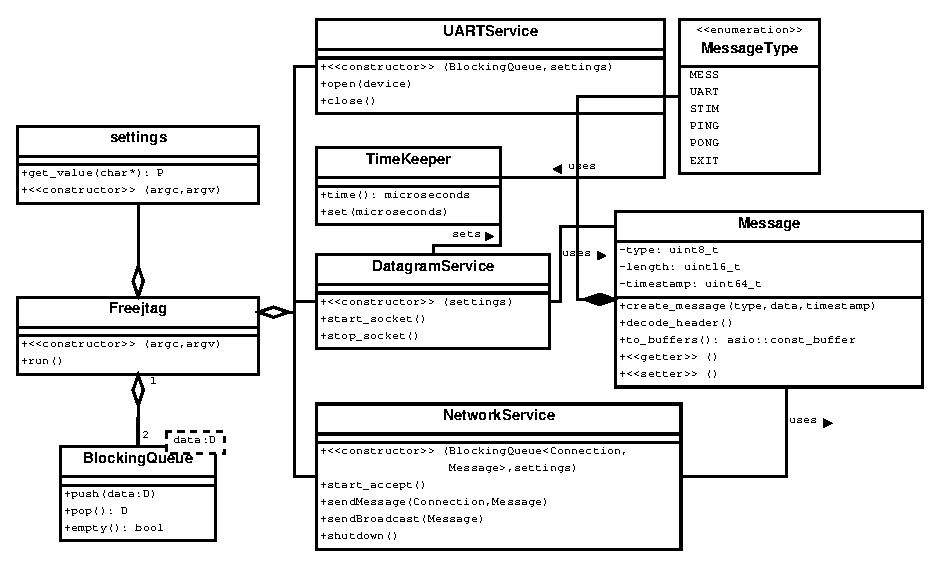
\includegraphics[width=\textwidth]{server.eps}
\caption{Grober Aufbau der Serveranwendung}{Diese Abbildung verdeutlicht den
Aufbau der Serveranwendung (\emph{FreeJTAG}). Hierbei wurden Details zu Gunsten der
Übersichtlichkeit ausgelassen.}
\label{fig:server}
\end{figure}
\autoref{fig:server} stellt eine grobe Übersicht über den Aufbau der
Serveranwendung dar. Hierbei wurden Details wie weitere Klassen und
zusätzliche Aggregationen zwischen den einzelnen Elementen zugunsten einer
besseren Übersicht ausgelassen.

Die Hauptanwendung \texttt{Freejtag} dient als "`Bindeglied"' zwischen den
einzelnen Bestandteilen der Software. Die genaueren Abläufe hierzu sollen in
\autoref{subs:abl} erläutert werden.

Weiterhin besteht die Serversoftware aus einer Klasse
\texttt{NetworkService} zur Übertragung der Nutzdaten, \texttt{DatagramService}
um die Zeitsynchronisation über UDP zu managen und \texttt{UARTService} für den
Empfang der Daten vom Zielsystem.

Die Klasse \texttt{Message} dient zum Parsen der Netzwerkdaten und wird somit
sowohl vom TCP- als auch vom UDP-Dienst verwendet.

Da die Zeitstempel synchronisiert werden sollen, wurde die Klasse
\texttt{TimeKeeper} erstellt. Sie dient dem Setzen der Zeitdifferenz und der
Abfrage des aktuellen Zeitstempels unter Berücksichtigung der gespeicherten
Differenz.

Die Hilfsklasse \texttt{BlockingQueue} wird als Schnittstelle zwischen dem
Hauptprogramm und dem \texttt{UARTService} sowie zwischen dem Hauptprogramm
und dem \texttt{NetworkService} eingesetzt. Sie ist nötig, da jeder dieser
Dienste in einem anderen Thread läuft und der Datenaustausch aus diesem Grund
synchronisiert werden muss.

\subsection{Funktionsweise der Serversoftware}\label{subs:abl}
In diesem Abschnitt sollen die wichtigsten Abläufe in der Serveranwendung
erläutert werden. Der Schwerpunkt liegt hierbei hauptsächlich auf der
Synchronisierung der Zeit und dem Weiterleiten der gesammelten Daten.
\subsubsection*{Programmstart}\label{subs:start}
Die Anwendung wird zuerst initialisiert und anschließend ausgeführt. Dies
erfolgt durch folgenden Ablauf.
\begin{lstlisting}[language=C++]
int main(int argc, char* argv[]) {
    freejtag::Freejtag *prog;
    prog = new freejtag::Freejtag(argc, argv);
    int res = prog->run();
    delete prog;
    return res;
}
\end{lstlisting}

Für die Funktion dieser Software müssen zu Beginn einige Einstellungen
festgelegt werden. Hierzu zählen die Parameter der \gls{uart}-Verbindung
(Baudrate, Parität, Stopp-Bit) und der Netzwerkport.

Bei Erstellung des \texttt{Freejtag}-Objektes werden zuerst die Werte aus
\listinlsh{/etc/freejtag.cfg} und die per Parameter (und in diesem Fall
Kommandozeile) übergebenen Argumente als Einstellungen eingelesen.
Das Einlesen dieser Werte erfolgt unter Nutzung der
\emph{Boost.Program\_options}-Bibliothek. Tritt hierbei ein Fehler auf, wird das
Programm mit einer Fehlermeldung beendet.

Intern werden die über das Netzwerk zu versendenden und empfangenen Nachrichten
mittels \listinlcpp{boost::shared\_ptr}(Smart Pointer) von
\texttt{Message}-Objekten verwendet. Es muss nun eine \\\texttt{BlockingQueue}
initialisiert werden, die die über den TCP-Port empfangenen Nachrichten
verwaltet. Da asynchrone TCP-Sendevorgängen mittels der
\listinlcpp{boost::asio}-Bibliothek erfolgen, ist eine weitere
\texttt{BlockingQueue} zur Synchronisierung hierfür nicht notwendig.

Da es möglich sein soll mehrere Verbindungen (Siehe auch \autoref{subs:best}) zu
verwalten, muss in der \texttt{BlockingQueue} zusammen mit der \texttt{Message}
auch immer die Verbindung von der sie erhalten wurde gespeichert werden.

Eine zweite \texttt{BlockingQueue} dient zur Erfassung der über \gls{uart}
gesammelten Daten mit zugehörigen Zeitstempeln. 

Nun werden sowohl \texttt{NetworkService} als auch \texttt{DatagramService}
initialisiert.

Der \texttt{NetworkService} erhält hierfür die vorher erstellte
\texttt{BlockingQueue}(den Buffer), legt das Protokoll auf TCP fest und
öffnet den in den Einstellungen spezifizierten Port. Der Ablauf des
\texttt{DatagramService} verläuft analog mit dem Unterschied, dass für die über
diesen Dienst erfolgende Zeitsynchronisation kein Zugriff auf den
Nachrichten-Buffer nötig ist.

Anschließend werden zwei Threads gestartet, die für die Abwicklung der, durch
den Empfang von \gls{uart}- oder Netzwerkdaten angestoßenen, Vorgänge
zuständig ist. Hierfür warten die Threads mittels \listinlcpp{UARTMessage msg =
input_uart_.pop();} beziehungsweise \newline\listinlcpp{MessageDatagram msgd =
input_network_.pop();} auf die Ankunft neuer Daten in ihrere zugehörigen
\texttt{BlockingQueue}. Dies schließt die Initialisierung ab.

Nun muss nun \listinlcpp{Freejtag::run();} aufgerufen werden, um den Start der
Anwendung zu vollziehen. Dies startet ein asynchrones Accept auf dem Socket des
Netzwerkmoduls, so dass es nun möglich ist, eine Verbindung zum Server
herzustellen. Der \gls{uart}-Anschluss wird auf dem angegebenen Gerät geöffnet
und mit den eingestellten Parametern konfiguriert.

Schließlich ruft der startende Thread die blockierende Methode
\listinlcpp{io_service_.run();} auf und dient nun zur Abarbeitung der
asynchronen Netzwerkvorgänge.

Damit ist der Programmstart abgeschlossen und die Serveranwendung kann nun
verwendet werden.
\subsubsection*{Zeitsynchronisation}
Der aktuell gültige Zeitstempel wird bei Aufruf von
\listinlcpp{Timekeeper::time()} durch eine simple Subtraktion errechnet.
\begin{lstlisting}[language=C++]
static high_resolution_clock::time_point epoch;
microseconds TimeKeeper::time(){
    high_resolution_clock::duration now = 
    			high_resolution_clock::now() - epoch;
    return duration_cast<microseconds>(now);
}
\end{lstlisting}
Um diese Berechnung durchführen zu können, muss jedoch zuerst eine
Synchronisation des Systems zum Client erfolgen. Der Ablauf dieser
Synchronistion erfolgt wie in \autoref{subs:time} beschrieben.

Der Einfachheit halber ist der Server nicht in der Lage, mehrere
Synchronisierungsvorgänge gleichzeitig durchzuführen. Diese müssen also
nacheinander ausgeführt werden.

Um die Abweichung zuverlässig ermitteln zu können, erfolgt nach 20
erfolgreichen Synchronisierungsvorgängen eine Bildung des arithmetischen Mittels
aller bis zu diesem Zeitpunkt gewonnenen Daten. 

Eine Ausnahme bilden hierbei Ergebnisse, die einen Differenz zum Client von mehr
als \SI{90}{\ms} aufzeigen. Tritt eine solch "`hohe"' Differenz auf, wird die
Abweichung unverzüglich und auf Basis dieses einen Ergebnis justiert. Hierdurch
soll einer Verfälschung der Mittelwertbildung durch anfänglich stark
abweichende Uhren vorgebeugt werden.

Da nun die gemittelte Abweichung zur Clientsoftware ermittelt wurde, kann die
Funktion \newline\listinlcpp{TimeKeeper::set(microseconds difference)} verwendet
werden, um die aktuell gültige \listinlcpp{epoch} anzupassen. Durch diese
Justierung wird der \texttt{TimeKeeper} effektiv auf \SI{0}{\micro\second}
gesetzt.

\subsubsection*{Empfang und Weiterleitung von UART-Daten}
Die Hauptfunktion des Servers liegt im Weiterleiten von über den
\gls{uart}-Anschluss erhaltenen Daten.

Ein beispielhafter Ablauf ist in \autoref{fig:serveruart} abgebildet.

Sobald die asynchrone Empfangsroutine des \texttt{UARTService} aufgerufen wird,
fragt diese den aktuellen Zeitstempel über den \texttt{TimeKeeper} ab. Zu
diesem Zweck besitzt dieser die statische Funktion \listinlcpp{time()}, die den
aktuellen Zeitpunkt in Mikrosekunden wie in \autoref{subs:servertime}
erläutert zurückgibt.

Anschließend wird der Zeitstempel zusammen mit der erhaltenen Textzeile in die
Buffer-Queue gegeben. Aus dieser Queue wird dieses Zeitstempel-Nachrichten-Paar
abgeholt und mittels \listinlcpp{NetworkService::sendBroadcast(Message::pointer
msg)} asynchron an alle verbundenen Clients gesendet.

Die Entkoppelung zwischen \texttt{UARTService} und \texttt{uart\_handle()}
mittels Buffer wird nötig, um das System möglichst modular zu halten. So wäre es
zum Beispiel eine Erweiterung um \gls{spi}-Funktionalität denkbar. Hierfür müsste
lediglich der gleiche Buffer an einen zu erstellenden \texttt{SPIService}
übergeben werden.

\begin{figure}
\centering
\begin{sequencediagram}
\newthread[0]{uart}{:UARTService}
\newinst[9pt]{time}{:TimeKeeper}
\newinst[9pt]{queueuart}{:BlockingQueue}
\newthread[9pt]{uartdisp}{uart\_handle()}
\newinst[9pt]{net}{:NetworkService}
\begin{call}{uart}{time()}{time}{timestamp}
\end{call}
\setthreadbias{west}
\begin{call}{uart}{push()}{queueuart}{}
\end{call}
\setthreadbias{center}
\prelevel{4}
\begin{call}{uartdisp}{pop()}{queueuart}{Data}
\postlevel{4}
\end{call}
\begin{call}{uartdisp}{sendBroadcast()}{net}{}
\end{call}
\end{sequencediagram}
\caption{Ablauf bei Empfang einer Zeile von \gls{uart}}{In diesem Ablauf
werden die Vorgänge nach Empfang einer Zeile des \gls{uart} dargstellt. Hierbei
ist zu beachten, dass der \texttt{UARTService}, anders als hier eingezeichnet,
keinen eigenen Thread besitzt. Stattdessen wird ein asynchrones
Ereignis ausgelöst.}
\label{fig:serveruart}
\end{figure}
\subsubsection*{Beenden des Servers}
Zum Beenden der Serveranwendung wird eine \texttt{EXIT}-Nachricht an den Server
geschickt.
%%\begin{minipage}[c]{\textwidth}
Dieser führt anschließend folgende Schritte aus:
\begin{itemize}
  \item Ausgeführt duch Thread \texttt{network\_dispatcher\_}
  \begin{itemize}
  \item Variable \texttt{\_running} auf \listinlcpp{false} setzen
  \item Acceptor für neu ankommende Verbindungen schließen
  \item Auf dem Socket der TCP-Verbindung ein \listinlcpp{socket\_.shutdown()}
  und \listinlcpp{socket\_.close()} ausführen, um die Verbindungen zu schließen
  \item Den Seriellen Port des \texttt{UARTService} mittels
  \listinlcpp{port\_.close()} schließen
  \item Den Socket des UDP-Servers mittels \listinlcpp{socket\_.close()}
  schließen
  \item Da keine Netzwerkoperationen anstehen, ist der Hauptthread nun nicht
  mehr auf  \listinlcpp{io\_service\_.run()} blockiert
  \end{itemize}
  \item Ausgeführt durch Hauptthread
  \begin{itemize}
    \item Den auf \listinlcpp{input\_network\_.pop();} blockierenden
    \texttt{network\_dispatcher\_} unterbrechen
    \item Den auf \listinlcpp{input\_uart\_.pop();} blockierenden
    \texttt{uart\_dispatcher\_} unterbrechen
  \end{itemize}
\end{itemize}
%%\end{minipage}
\section{Client - The Kraken}
\begin{figure}[!ht]
\centering
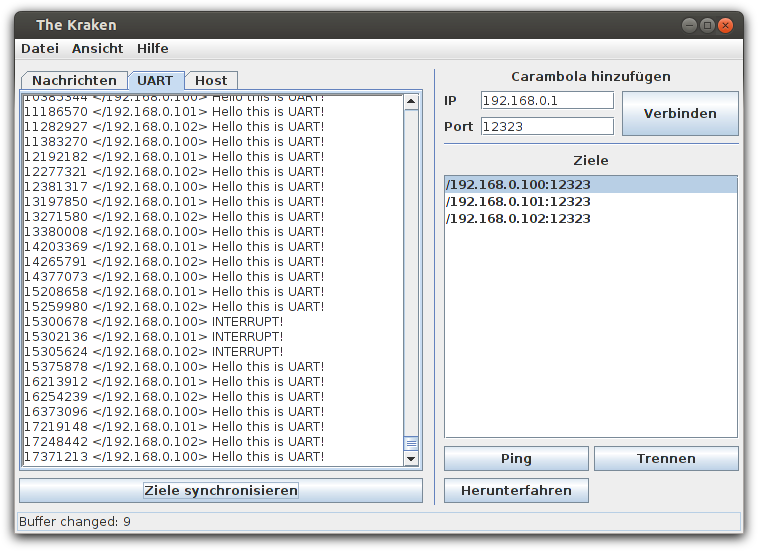
\includegraphics[width=\textwidth]{client.png}
\caption{Die Clientanwendung}{Diese Abbildung zeigt die Clientanwendung
"`The Kraken"' beim Erfassen der gesammelten Daten. Ein bei den
Zielsystemen gleichzeitig ausgelöster Interrupt ist erkennbar.}
\label{fig:client}
\end{figure}
\subsection{Funktionalität}
Die Clientsoftware dient dem Erfassen und Anzeigen der von der Serversoftware
gesammelten Daten. \autoref{fig:client} stellt die Oberfläche der Software dar.

Die Software erfüllt folgende Funktionen:
\begin{itemize}
  \item Verbindungsaufbau zu einer beliebigen Anzahl Server
  \item Sortierung der Daten. (Siehe \autoref{subs:sort})
  \item Beenden einer Serveranwendung
  \item Senden von \texttt{MESS}-Nachrichten an einen Server (Broadcast)
  \item Unterbrechen der Datenaufnahme
  \item Synchronisieren der Zeiten aller Serveranwendungen mit dem Client
  \item <weitere Funktionen> 
\end{itemize}
\subsection{Aufbau der Anwendung}
Die Strukturierung der Clientanwendung folgt lose dem \gls{mvp}-Modell.

<!!!AUSFÜHRLICHER!!!>

Der EventBus der \emph{Google Guava}-Bibliothek wird verwendet, um die
Ereignisse der Softwareelemente miteinander zu verknüpfen.

Die Anwendung wurde mithilfe des Build-Management-Tools "`Maven"'
entwickelt.
\subsection{Sortierung der Daten}\label{subs:sort}
Da die Daten im Betrieb fortlaufend eintreffen, wird eine entsprechende Methode
benötigt, die Daten zu sortieren.

Ein Sortieralgorithmus wie zum Beispiel "`Quicksort"' funktioniert nur so lange,
wie die Daten konsistent bleiben. Da sie das in diesem Fall jedoch nicht sind,
ist nach einer alternativen Lösung zu suchen.

Ein \textbf{TreeSet} sorgt dafür, dass die Daten direkt beim Eintreffen nach
ihren Zeitstempeln in den Baum einsortiert werden. Dies erlaubt es relativ
einfach, das jeweils kleinste Element (das Element mit dem niedrigsten
Zeitstempel) auszugeben. 

Hierbei muss jedoch sichergestellt werden, dass immer eine Anzahl an Nachrichten
in diesem Buffer verbleibt. Die Größe des Buffers beträgt aus diesem Grund
$\mathit{AnzahlVerbindungen}*3$.

\section{Deployment}
Mittels einer Linux-Scriptdatei lässt sich der \gls{gdb} im Batch-Modus steuern.
Zum Einsatz kommt hier ein Here-document, dass die in \autoref{subs:eclipse}
erwähnten Initialisierungsbefehle ausführt, um anschließend die Firmware durch
Ausführen von \listinlsh{load} zu flashen.
\begin{lstlisting}[language=sh]
#!/bin/bash
echo "Flashing $1"
for target in "${@:2}"
do
 echo "Flash $target"
 arm-none-eabi-gdb $1 <<EOF
 target remote $target:3333
 monitor reset halt
 monitor soft_reset_halt
 monitor wait_halt
 monitor poll
 monitor flash probe 0
 monitor soft_reset_halt
 tbreak main
 load
EOF
done
\end{lstlisting}
Dieses Script erfordert als erstes Argument die zu flashende Datei und
anschließend eine beliebige Anzahl von Zielsystemen.

Das Zurücksetzen der Zielsysteme erfolgt analog hierzu. Dabei entfallen jedoch
die Initialisierungsbefehle und das Flashen. Lediglich der Befehl
\listinlsh{monitor reset run} muss von gdb ausgeführt werden.

Die Einbindung in Eclipse ist durch die Verwendung der Scripte als "`Externe
Tools"' einfach möglich.
\section{Aufgetretene Probleme}
Während der Inbetriebnahme von \emph{OpenOCD} traten häufig Probleme mit der
Verbindung zum \gls{jtag}-Adapter auf. Dies äußerte sich darin, dass das
Linux-System regelmäßig die Verbindung zu dem Adapter verlor. Dies
erschwerte den Betrieb von \emph{OpenOCD} erheblich.

Jedoch ist dies, laut dem Benutzerforum des Herstellers, ein bekanntes
Konstruktionsproblem der "`Carambolas"' hervorgerufen durch eine unzulängliche
Schirmung des USB-Anschlusses gegenüber Elektromagnetischen Wellen.
Dies bewirkt, dass die integrierte WLAN-Antenne den Betrieb von USB-Geräten
unter Umständen stark beeinflusst.

Um dieses Problem zu beheben wurde ein \SI{32}{\mm} langer Draht an die Masse
der WLAN-Antenne gelötet. Anschließend lies sich der \gls{jtag}-Adapter
problemlos betreiben. Alternativ hätte auch die Möglichkeit bestanden, die
Sendeleistung des WLAN-Moduls über die Einstellung \listinlsh{option txpower 10}
in der Datei \listinlsh{/etc/config/wireless} zu reduzieren.
\section{Analyse des Systems}
Da die Präzision der Zeitstempel von zentraler Bedeutung für die
Aussagekraft der gesammelten Daten ist, muss festgestellt werden, wie exakt zum Beispiel die
Zeitsynchronisation funktioniert.

Um die Genauigkeit messen zu können, müssen alle Zielsysteme möglichst
zeitgleich ein Signal erhalten, um dann unverzüglich über \gls{uart} eine
Nachricht an die angeschlossenen "`Carambolas"' zu übermitteln.

Hierfür wurde exemplarisch das \gls{rtos} ChibiOS/RT\cite{CHIB} auf den
Zielsystemen installiert. Es wurde so konfiguriert, dass ein Interrupt ausgelöst
wird, sobald ein bestimmter Pin als "`Auslöser"' auf Masse gezogen wird.

Da die "`Carambolas"' durch separate Netzteile alle verschiedene Massepotentiale
haben, müssen diese zuerst miteinander verbunden werden. Anschließend kann man
alle "`Auslöser"'-Pins miteinander verbinden. Dies erlaubt es einem, mittels
eines Knopfes oder eines Überbrückungskabels, die so verbundenen Pins zeitgleich
auszulösen.

Hat man vorher einen Synchronisierungsvorgang durch den Client durchgeführt,
lässt sich durch die Differenz der Zeitstempel nun die tatsächliche Abweichung
voneinander messen. Im Idealfall ist die Differenz hierbei möglichst gering
(Nach \autoref{subs:time} weniger als \SI{1}{\milli\second}). Das Eintreffen
dieser erwähnten Interrupts ist auch auf \autoref{fig:client} zu erkennen.

Allerdings kann dies natürlich nur die Differenzen der Zielysteme untereinander
aufzeigen. Die Abweichung gegenüber dem Entwicklerrechner ist für eine Analyse
der Netzwerkabläufe jedoch auch von untergeordneter Relevanz, da dieser in den
Abläufen keine Rolle spielt.

\begin{figure}
\centering
\begin{tabu}{r|r r|r r | r}
& \multicolumn{2}{c|}{\textbf{Knoten 0}} & \multicolumn{2}{c|}{\textbf{Knoten
1}} & \textbf{Knoten 2}\\ \cline{2-6}
Minute & Zeitstempel & Diff zu Knoten 1& Zeitstempel &
Diff zu Knoten 2& Zeitstempel \\ \hline
0  & 10613705   &-0.02\ms & 10613684   &  0.2\ms & 10613859   \\
15 & 950992475  &  6.4\ms & 950998898  & 12.5\ms & 951011363  \\
30 & 1854818581 & 12.6\ms & 1854831162 & 24.3\ms & 1854855460 \\
45 & 2754582459 & 18.7\ms & 2754601202 & 36.2\ms & 2754637360 \\
60 & 3655782708 & 24.9\ms & 3655807605 & 47.9\ms & 3655855473 \\
75 & 4554104959 & 31.0\ms & 4554135948 & 59.6\ms & 4554195595 \\
90 & 5453785960 & 37.0\ms & 5453823040 & 71.5\ms & 5453894583 \\ \hline
& \multicolumn{2}{p{4,7cm}}{\textbf{Drift pro \SI{15}{\minute}
gegenüber Knoten 1}} & \multicolumn{2}{|p{4,7cm}|}{\textbf{Drift pro
\SI{15}{\minute} gegenüber Knoten 2}} &
\\
& \multicolumn{2}{c}{\textbf{\SI{6,2}{\ms}}} &
\multicolumn{2}{|c|}{\textbf{\SI{11,9}{\ms}}}&
\\
\end{tabu}\\
\caption{Testdaten einer Testreihe zur Prüfung der Genauigkeit der
"`Carambolas"'}{Die Zeitstempel sind die von der Clientsoftware
ausgegebenen Werte. Die Differenzen zwischen den Knoten sind gerundete Angaben,
da eine Genauigkeit der Zeitstempel von \SI{1}{\micro\second} nicht zu
erwarten ist. Der durchschnittliche Drift über \SI{15}{\minute} errechnet sich
über die Differenz zwischen den einzelnen Knoten nach einer Testzeit von
\SI{90}{\minute}.}
\label{fig:testtab}
\end{figure}

Es wurde ein Testtlauf über \SI{90}{\minute} durchgeführt. Direkt vor dessen
Durchführung wurde eine Zeitsynchronisation des gesamten
Entwicklungssystems und damit aller "`Carambolas"' durchgeführt.

Im Versuchsablauf wurde, wie weiter oben erläutert, ungefähr alle
\SI{15}{\minute} ein Interrupt bei allen Zielsystemen gleichzeitig ausgelöst.
Bei diese Testreihe war nicht entscheidend, den Interrupt exakt alle
\SI{15}{\minute} auszulösen, da hauptsächlich die sich verändernden Differenzen
gezeigt werden sollten.

Wie aus \autoref{fig:testtab} ersichtlich, ist direkt nach der Synchronisation
die absolute Differenz zwischen "`Knoten 0"' und "`Knoten 1"' bei nur
\SI{21}{\us} und zwischen "`Knoten 1"' und "`Knoten 2"' bei \SI{175}{\us}. Dies
zeigt, dass die Zeitsynchronisation eine ziemlich hohe Genauigkeit erreicht.

Aus dem Verlauf der Testreihe ist jedoch auch ersichtlich, dass die Differenz
zwischen den Systemen nicht gleichbleibend ist. So steigt über einen Zeitraum
von \SI{15}{\minute} die Differenz zwischen "`Knoten 0"' und "`Knoten 1"' um
ungefähr \SI{6,180}{\ms} und zwischen "`Knoten 1"' und "`Knoten 2"' um
\SI{11,924}{\ms}.

Dies erklärt sich aus den Fertigungstoleranzen der Schwingquarze. Die Abweichung
zwischen "`Knoten 0"' und "`Knoten"' vergrößert sich alle \SI{15}{\minute} um
ungefähr \SI{18}{\us} was einer Abweichung von 20 ppm entspricht
($\frac{\SI{18}{\us}}{\SI{15}{\minute}}*1000000=20\mathit{ppm}$).
Diese Abweichung ist für einen Schwingquarz noch innerhalb der üblichen
Frequenztoleranz.

Die Genauigkeit der Zeitsynchronisation selbst jedoch liegt in der in
\autoref{subs:time} geforderten Genauigkeit von ungefähr \SI{1}{\ms}.

\chapter{Ausblick}
\lipsum

%%%%
%% add some text to generate a sample document
%\chapter{Sample Chapter}

%\lipsum

%%%%

%% appendix if used
%%\appendix
%%\typeout{===== File: appendix}
%%\chapter{Installationshinweise}
Die beigelegte CD enthält den Quellcode der im Rahmen dieser Bachelorarbeit
entwickelten Software.

Da die Serversoftware stark in das Build-System von OpenWRT integriert
ist, folgt eine Auflistung der selbstentwickelten oder modifizierten Dateien.
\vspace{1pt}
\dirtree{%
.1 Hauptordner.
.2 Thesis.pdf Installation.
.2 scripts.
.3 flash-all run-all.
.2 binary.
.3 TheKraken.exe.
.3 chibios.elf.
.3 openwrt-ramips-rt305x-carambola-squashfs-sysupgrade.bin.
.2 thekraken.
.3 src.
.4 \ldots.
.3 pom.xml.
.2 chibios.
.3 \ldots.
.2 carambola.
.3 package.
.4 freejtag.
.5 files.
.6 freejtag.uci-defaults openocd.cfg openocd.init. 
.5 src.
.6 \ldots.
.5 Makefile.
.4 openocd.
.5 Makefile.
.3 feeds/packages/libs/libftdi.
.4 Makefile.
}
\vspace{1pt}
Alle weiteren Dateien sind ausdrücklich nicht Bestandteil dieser Arbeit,
allerdings für die Verwendung der Software notwendig.
In der Datei \texttt{Installation} befinden sich Hinweise zur Konfiguration des
Entwicklersystems und zum Kompilieren eines OpenWRT Images.

% bibliography and other stuff
%\backmatter

\typeout{===== Section: figures}
\listoffigures

\typeout{===== Section: literature}
%% read the documentation for customizing the style
%%\bibliographystyle{dinat}
%%\bibliography{sample}
\printbibliography[heading=bibintoc]

\typeout{===== Section: nomenclature}
%% uncomment if a TOC entry is needed
%%\addcontentsline{toc}{chapter}{Glossar}
\renewcommand{\nomname}{Glossar}
\clearpage
\markboth{\nomname}{\nomname} %% see nomencl doc, page 9, section 4.1
\printnomenclature

%% index
\typeout{===== Section: index}
\printindex

\HAWasurency

\end{document}
